\section{A summary of knot presentations}\label{sec:notation} % (fold)


The knot presentations we focus upon herein are the Gauss code \cite{Read1977On-the-Gauss-cr}, the
Dowker-Thistle\-thwaite (DT) code \cite{DT}, the Conway notation \cite{Conway1970An-enumeration-}, and the Master
Code of Rankin, Schermann and Smith \cite{Rankin2004Enumerating-I} \cite{Rankin2004Enumerating-II}. Other presentation schemes, such
as braid representatives and Morse links, are not directly useful to
the development of this paper and thus are overlooked. We also give a
``wish-list'' of properties one would desire from one's knot notation
scheme.

\subsection{Knot presentations}
This section briefly discusses various knot notations and establishes
some terminology, with references for readers needing further details.

\subsubsection{Regular knot projections}

In 1847, J.B. Listing classified knots up to 5 crossings by analyzing
knot projections \cite{Listing1848Vorstudien-zur-}. Listing was the
first to publish an article containing a drawing of a regular knot
projection (or \emph{knot diagram} or \emph{planar diagram}). A
\emph{knot} is taken to be a polygonal simple closed curve in
$3$-space. Choose any plane on which projection onto the plane results
in a curve whose only singularities are transverse double points which
are not the image of any vertex from the polygonal curve. Using a
canonical normal vector to the plane for line of sight, for a given
double point $d$ we find the point $c$ in the projection's preimage of
$d$ farthest from our line of sight, and we indicate an undercrossing
by erasing the image of a small neighborhood of $c$ from the planar
projection. A careful presentation is given in \cite{LivingstonText}.
	
Out of all possible regular projections of a knot, there is (at least)
one with minimal number of crossings. 

% We'll write $\#(K)$ to denote this number.


\subsubsection{The Gauss code.} Gauss used regular knot projections to
arrive at what is now called the Gauss Code of a knot
\cite{Read1977On-the-Gauss-cr}. The Gauss code is the first knot notation
system. P. G. Tait used an encoding in the 1870's to classify knots up
to 7 crossings \cite{Tait}. Tait's encoding may be regarded as an
extension to the Gauss Code. One begins somewhere on the knot
projection (not at a crossing point), then proceeds along the knot
applying labels to the first, third, fifth etc. crossing until all
crossings are labeled; one then traverses the knot once more, writing
the label of each crossing in the order that you reach it, attaching a
plus or minus sign, depending on whether you are crossing over or
under.

\subsubsection{Tait, Little, and Kirkman.} Using Kirkman's
classification of certain polygons \cite{Kirkman1885The-enumeration},
Tait (and Little, using similar methods) was able to tabulate knots up
to 11 crossings \cite{Tait} \cite{Little1885On-knots-with-a}
\cite{Little1890Alternate-pm-kn}
\cite{Little1900Non-alternate-p}. Tait's system included using a
simple reduction rewrite strategy within his notation system. This notation was improved by Dowker and Thistlethwaite, as discussed in some detail below.



\subsubsection{Reidemeister moves.} Reidemeister developed a reduction
rewrite system for knot projections (“the three Reidemeister moves”)
\cite{ReidemeisterMoves}. We illustrate the three moves. The
convention in these (and in other graphically-based invariants) is
that we show only the relevant part of the knot. In our diagrams here,
we have placed dashed circles, which the reader should imagine as
viewing through scope lens only a portion of the knot, with
the remainder of the knot outside of the scope of view and unchanged.

\begin{figure}[hbt]
    \centering
    \scalebox{0.37}[0.370]{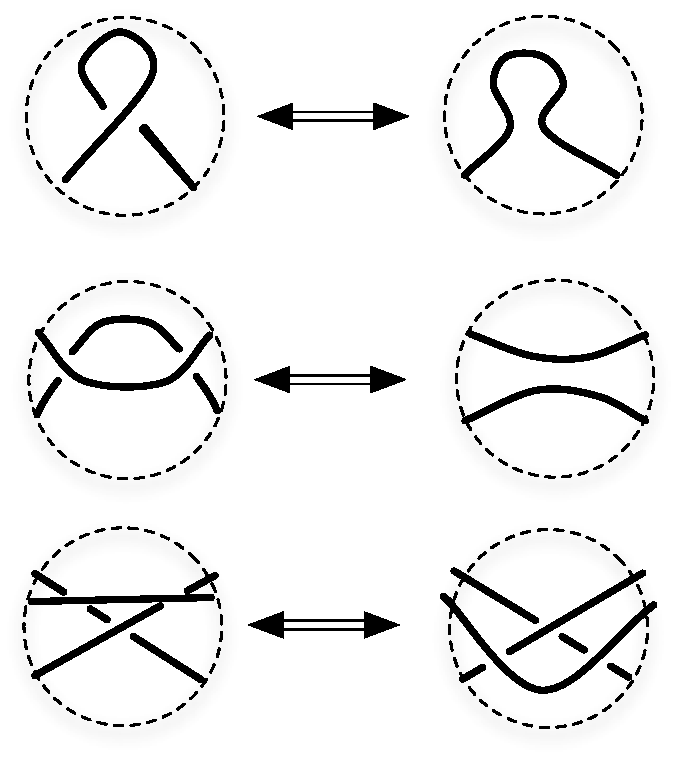
\includegraphics[viewport=0 0 390 360]{../../illustrations/Reidemeister123vert.pdf}}
    \caption{ The three Reidemeister moves. The topmost move will be referred to as $R_1$, the middle one as $R_2$, and the bottommost as $R_3$. For any one of these moves $R$, we write $R^{\to}(K)$ (resp. $R^\leftarrow$(K)) if the move has been applied left-to-right (resp. right-to-left)  to the knot diagram $K$.}
\label{fig:RMoves}
\end{figure}

The import of this system is Reidemeister's Theorem: an ambient
isotopy of two knots may be exhibited as sequences of rewrites of (any of) their
diagrams, and vice versa. That is, two knots are ambient isotopic if and only if a
diagram of one may be rewritten, via a sequence of Reidemeister
moves, to a diagram of the other \cite{LivingstonText}.



\subsubsection{Knotation} Conway developed a clever notational system
for tangles, finding an algebraic-like system for this system that led to several methods of reduction rewrites
\cite{Conway1970An-enumeration-}. He used this system to retabulate
knots and links of 11 crossings by hand, in one afternoon (an effort
that took Tait and Little years of work), discovering one omission and
a few duplications in the process. Conway's system can be used to
classify all arithmetic (also called algebraic, or rational)
knots. The Conway code for a knot originally was given as a “basic
polyhedron” followed by a sorted list of arithmetic tangles. See
Conway's paper \cite{Conway1970An-enumeration-} for details. This system has extensions by Caudron
\cite{Caudron1981-Classification} and by Bangert
\cite{Bangert2002Algorithmic-Pro}. Conway has investigated further
structures such as bangles and bracelets.

\subsubsection{Dowker-Thistlethwaite Codes (DT codes)}\label{ssub:dowker_thistlethwaite_codes} % (fold)
Dowker created a variation of Tait's notational system that is easier
to implement computationally. Dowker and Thistlethwaite made it the
basis for an algorithm that successfully enumerated knots of up to 13
crossings \cite{DT}. Not every DT code is valid, i.e. an arbitrary DT
code may not correspond to an actual knot, and two distinct composite
knots may share the same DT Code. However, a valid DT code for a prime
knot specifies the knot uniquely \cite{SchareinPhD}. In their paper,
Dowker and Thistlethwaite develop an algorithm to filter out invalid
cases. They also give a reduction system to remove duplicates from
their enumeration.

We now recall the definition of the DT code of
a regular knot projection \cite{DT}. Begin at a selected point on the
diagram (excepting crossing points) and traverse the diagram in a
selected direction. At each encounter of a crossing, label the
crossing with the next available counting number; for an even label,
prepend a negative sign if traversing the overcross. Returning to the
beginning point, each crossing has been labeled twice, once with an
odd number and once with an even number. Let $S_\pm$ denote the set of
labels generated.

If the knot projection has $n$ crossings, then there are $2n$ labels
(from $1$ to $2n$ in absolute value) and at each crossing an unique
odd counting number paired with an even integer. This induces a
parity-reversing function $\sigma$ on $S= \{1,\ldots,2n\}$, where for
each $i\in S$ we find the crossing with label whose absolute value is $i$ and let
$\sigma(i)$ be the absolute value of the other label at that crossing.
Note that $\sigma(\sigma(i))=i$ for any $i\in S$. Note that there is
also a bijective translation $\tau: S\to S_\pm$ where
$\abs{\tau(s)}=s$ for all $s\in S$.  Then the DT code of the knot
projection is determined by $\delta=\tau\circ\sigma$, usually given as
the list $\{\delta(1),\delta(3),\ldots,\delta(2n-1)\}$. Note that
$\delta\circ\sigma=\tau$. Finally, for each $i\in S$, let $sgn(i)$
denote the sign of $\tau(i)$ (so $sgn(i)<0$ implies $i$ is even).

For each $i\in S_\pm$, let $C(i)$ denote the crossing with label
$i$. Then for any $i\in S$ we know $C(i)$ is adjacent to the two
crossings $C(i\pm 1)$ and $C(\delta(i)\pm 1))$, where addition is modulo $2n$. This fact is applied
later when giving an explicit algorithm for encoding a knot.


% subsubsection dowker_thistlethwaite_codes (end)
 
\subsubsection{From Calvo to Rankin, Flint, and Schermann} Calvo
developed an inductive knot tabulation algorithm, thereby sidestepping the need to
check validity of DT codes \cite{Calvo1997Knot-enumeratio}. However, detection of
duplication within the tables generated then becomes the issue. Calvo had the insight that
understanding the deeper flype structure of prime, non-alternating
diagram led to greater efficiencies in his algorithm. The Calvo
algorithm was essentially refined in the development of a notational
system by Rankin, Flint, and Schermann , based on what they call
the group code which reminds one somewhat of the Gauss code but, instead, using a
Conway-like insertion scheme to allow for easy reduction of flype
structures in the notation \cite{Rankin2004Enumerating-I}
\cite{Rankin2004Enumerating-II} \cite{Rankin2004EnumeratingLinks}. This results in a master array that provides a unique identifier for  prime alternating knots. This forms part of the basis for inductive construction of all prime alternating knots of crossing size $n$ from those of crossing size $n-1$(see the above papers for details).  Composite knots remain problematic, due principally to the issue of detection of duplicates.




\subsection{Desirable properties for a knot presentation system }\label{sub:desirable_properties_for_a_knot_notation_system_} % (fold)

In this section, we list some properties that one would wish for a
knot presentation system to enjoy, followed by a discussion of the
knot presentations of the last subsection in the light of these
wishes.

Due to complexity considerations, one may well despair of a knot
notation system that would allow for mathematical classification of
all knots. However, in designing a system of knot notation or
presentation, informed by the history of knot tabulation and
classification we can enumerate the following properties such a
notation system may enjoy. These properties invariably correspond to
demands of functoriality on the encoding when considered as a map from
the category of knots or braids to some suitable target category while
others are demands on the faithfulness (respectively, fullness) of the
encoding considered as functor.

\begin{itemize}


\item {Surjection (realizability).} Each code in the notation represents
  a knot (or if this is not the case, those codes that do not
  represent a knot are easily recognizable). A code for a knot should
  be easily obtained from one of its planar diagrams.

%\item [Reduction] 
\item {Reduction.} The notation enjoys a calculus with which to reduce
  and simplify encodings. Each step of simplification or reduction
  results in an encoding representing a knot isotopy equivalent to the
  originating knot.

%\item [Minimality] 
\item {Minimality.} The notational encoding of a given knot can be
  reduced to a (finite non-empty set of equivalent) minimal
  encoding(s).

%\item [Injection] 
\item {Well-definedness.} If a knot has two (or more) minimal reduced
  encodings, each of these encodings is equivalent to the notation for
  a knot equivalent \emph{via} ambient isotopy to the original.

\item {Injection.} Two knots that have equivalent
  minimal reduced encodings are ambient isotopic.


	\item {Economy.} The notation is computationally cheap and easily constructed from a diagram of the knot or from a simple code, such as the DT code.
	
%\item [Compositionality] 
\item {Compositionality.} Operations on knots, e.g. knot
  composition, correspond to natural operations on elements in the
  image of the encoding.
  
%\item [Separation] 
\item {Separation.} The notation can be used to classify a class X of
  knots, where X contains a previously classified class of knots (for
  example, arithmetic knots (also known as algebraic knots) and
  bracelets) but is not previously classified itself.

%\item [Classification] 
\item {Extensibility.} The notation enjoys a formal language in which
  to describe properties and invariants of notation objects that
  reflect interesting properties of knots. This language should also
  be useful in selecting specific sets of knots (such as the set of
  all 21-crossing prime alternating links containing the tangle
  5/3). This language ideally should be scaleable and be applicable to
  tables of indefinite size.
\end{itemize}

The DT code, with proper care taken, satisfies the
first six properties but breaks under compositionality. Conway's
tangle notation enjoys all of the properties listed, though the Conway
encoding requires foreknowledge of the classes of basic polygons with
$n$ vertices. The master array of Rankin, Flint, and Schermann 
satisfies the first five properties, but appears unlikely to support
the last four properties to a degree useful for anything other than
tabulation.

\subsubsection{A meta-knotation}

 Due to Reidemeister's Theorem, in order to establish our main theorem we need only consider diagrams of knots and not knots themselves. Hence we  adopt the following convenient
notation and terminology. The meta-variable  $K$
ranges over knot diagrams and we reserve $\mathcal{K}$ to range over knots. For simplicity, we refer to $K$ as a knot. We write $\#(K)$ to mean the number of crossing points in the diagram $K$ but will call this value the crossing number of the knot $K$, which the reader is asked not to confuse with the minimal crossing number of the knot (it is in this sense that we will later say that ``two knots from the same isotopy class can have different crossing numbers'').   Formally speaking $\sim_{\text{iso}}$ will denote  equivalence of knots under ambient
isotopy and $\sim_{R}$ will denote equivalence of diagrams under (finite) sequences of
Reidemeister transforms. However, when there is little chance of confusion we
drop the subscript and write $\sim$.  

% subsection desirable_properties_for_a_knot_notation_system_ (end)

% section notation (end)